\section{Feature Learning}
In this section, we take a re-look at the NTK and NTK matrices, and explicitly write down the terms related to feature learning.\hfill\\
\textbf{ReLU artefact or NTF vs NPF:} Recall that the neural tangent feature is given by $\psi_{x,t}=\phi^\top_{x,t} {\partial} v_t + {\partial} \phi^\top_{x,t} v_t$. We note that, in the case when $A_t(x,p)\in\{0,1\}$ (such as in DNN with ReLU activations)  $\partial_{\phi}=0$, and hence is not accounted for in the SGD update as well as in the trajectory analysis. However, due to the SGD update, the gating value changes during training, and consequently the activations, the NPF, the NPK change during training as seen in the experiments in \Cref{sec:generalisation}. We side step this artefact by studying network with soft-gates: given a pre-activation input, a hard gate (uch as ReLU) uses $\mathbbm{1}_{\{q>0\}}$, while a soft-gate uses a soft-max sigmoidal function $\chi_\epsilon(q)=\frac{1+\epsilon}{1+\exp(-\beta q)}$. We consider sofr-ReLU networks denoted by $\N_{SR}(\Theta_t)$, and soft-GaLU networks denoted by $\N_{G}(\Theta_t, \G(\N_{SR}(\Tg_t)))$. We checked the performance of soft-gates by training, a soft-GaLU network and a soft-ReLU network, and the fact that adaptable gates generalise better than frozen gates continued to hold (see \Cref{fig:gen} which shows the performance of all the $4$ networks namely ReLU, frozen-GaLU, soft-GaLU and soft-ReLU).\hfill\\
\textbf{NTK and feature learning:} In the case of  soft-GaLU networks, since there are two set of parameters (total $2d_{net}$), we have the neural tangent feature to be $\psi_{x,t}=[\psi^v_{x,t},\psi^a_{x,t}]=[\partial_{\Theta} \hat{y}_t, \partial_{\Tg} \hat{y}_t]\in \R^{2d_{net}}$. Thus the NTK matrix is given by $K_t=K^w_t+K^a_t$,  where $K^w_t={\Psi^v_t}^\top \Psi^v_t$, and $K^a_t={\Psi^a_t}^\top \Psi^a_t$, where $\Psi^v_t=[\psi^v_{x_s,t},s\in[n]]$ and $\Psi^v_t=[\psi^a_{x_s,t},s\in[n]]$ are the NTF matices. In the case of  soft-ReLU networks, i.e, $\N_{SR}(\Theta_t)$  it is easy to check that $K_t={K^v_t}+{K^a_t}+{\Psi^v_t}^\top {\Psi^a_t}+{\Psi^a_t}^\top {\Psi^v_t}$.
\begin{definition}\label{def:delta}
For a soft-GaLU networks, using any $i\in[d_{in}]$, define $\delta_t(s,s')\stackrel{def}= \underset{{p\rsa i}}{\sum} \sum_{\tg\in\Tg}\frac{\partial A_{t}(x_s,p)}{\partial \tg} \frac{\partial A_{t}(x_{s'},p)}{\partial \tg}$.
\end{definition}
\begin{lemma} Under \Cref{assmp:main}, in soft-GaLU networks we have: (i) $\E{K_0}=\E{K^w_0}+\E{K^a_0}$, 
 (ii) $\E{K^w_0}=\sigma^{2(d-1)} (x^\top x)\odot \lambda_0$,  (iii) $\E{K^a_0}=\sigma^{2d}  (x^\top x)\odot \delta_0$
\end{lemma}
\textbf{Discussion}: \hfill\\
$1.$ Note that in \Cref{def:delta}, $\delta_t$ contains $\partial A_t(x,p)$ terms as opposed to $A_t(x,p)$ term in $\lambda_t$ defined in \Cref{def:lambda}. For a path $p$, if a path contains gates that are very close to either $0$ or $1$, then $\partial A_t(x,p)$ will be very small. Since $\frac{\partial A_{t}(x_s,p)}{\partial \tg}= \sum_{l=1}^{d-1} \Big(\frac{\partial G_{x_s,\Tg_t}(l,\I_l(p))}{\partial \tg} \Big)\Big(\Pi_{l'\neq l} G_{x_s,\Tg_t}(l',I_{l'}(p))\Big)$, for a path $p$ containing $d-1$ gates close to $1$, and only one gate whose pre-activation input is close to $0$ will have a significant $\partial A_t(x,p)$. \hfill\\
$2.$ Let us take the case of classification with cross-entropy loss. Now, say we have trained till some $T$ epochs with good classification (say close to $100\%$) accuracy. Considering the fact that $\hat{y}_T=\Phi_{\Tg_T}v_{\Theta_T}$, the gradient with respect to $\Tg$ will change the NPF matrix $\Phi_{\Tg_T}$ in such a manner to reduce the loss, i.e., increase the margin of each of the classified examples, subject to the `well-conditioned' ness of $K^a_T$. While this scenario is idealistic, in practice, both $\Tg_t$ as well as $\Theta_t$ change, and we need to understand how the joint optimisation and feature learning happens.\hfill\\
\begin{figure}[h]
\resizebox{\textwidth}{!}{
\begin{tabular}{cccc}
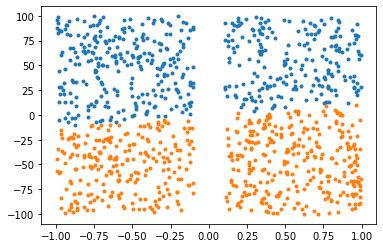
\includegraphics[scale=0.2]{figs/simple-original.png}
&
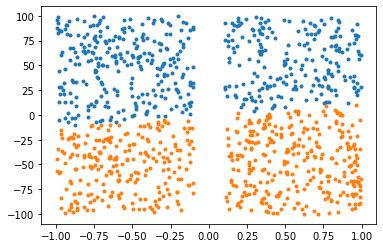
\includegraphics[scale=0.2]{figs/simple-feat.png}
&
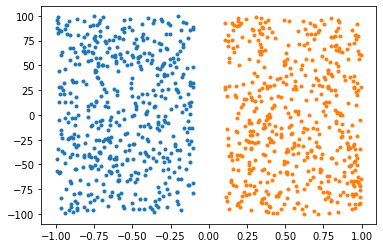
\includegraphics[scale=0.2]{figs/adapt-original.png}
&
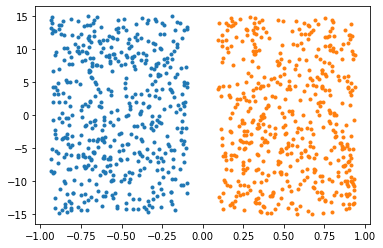
\includegraphics[scale=0.2]{figs/adapt-feat.png}
\end{tabular}
}
\caption{From the left: First two plots show the performance on the training set with original ($x_s$) and internal features ($\phi_{x_s,t}$) in the case of frozen-gates. The third and fourth plots show performance on the training set with original ($x_s$) and internal feature ($\phi_{x_s,t}$)  in the case of adaptable gates.}
\label{fig:feat}
\end{figure}

\textbf{Toy Experiment:} We check the performance of frozen-gates versus adaptable gates in a toy experiment. The dataset is $(x_s,y_s)_{s=1}^{n},n=1000$, wherein, for $s=,1,\ldots,500$, $x_s(1)\stackrel{iid}\sim U[0.1,1]$, and $x_s(2)\stackrel{iid}\sim U[-100,100]$, and $y_s=1$, and for $s=501,\ldots,1000$, $x_s(1)\stackrel{iid}\sim U[-0.1,-1]$, and $x_s(2)\stackrel{iid}\sim U[-100,100]$, and $y_s=-1$. We transformed the input $x\in \R^2$ into a feature vector $\phi_{x,t}=(x(1)G_t(1),x(2)G_t(2) )\in \R^2$, where $G_t(i)=\frac{1}{1+\exp(-\tg(i))},i=1,2$. The predicted output is $\hat{y}_{t}(x_s)=\phi^\top_t\Theta_t$, where $\Theta_t\in \R^2$. We use the loss function $L_t=\frac{1}{n}\sum_{s=1}^n\frac{1}{1+exp(-y_s\hat{y}_t(x_s)}$, and trained the model for $T=1000$ epochs, for the following two cases: i) frozen-gates, wherein, we set $\Tg_0=(10,10), \Tg_t=\Tg_0,\forall t\geq 0$, so that the input features are not transformed, and used gradient descent with stepsize $0.1$ to train $\Theta$ ii) adaptable gates, wherein, we performed gradient descent with stepsize equal to $0.1$ to train both $\Tg$ and $\Theta$. The results are shown in \Cref{fig:feat}, notice that the right most plot shows that in the case when the gates are adapting, they learn to suppress the second co-ordinate (the scale of $\phi_{x_s,T}$ is from $-15$ to $15$ as opposed to $-100$ to $100$ in $x_s$). 